\documentclass{beamer}

\input{preamble.tex}
\usepackage{breqn} % Breaks lines

\usepackage{amsmath}
\usepackage{mathtools}

\usepackage{pdfpages} % \includepdf

\usepackage{listings} % R code
\usepackage{verbatim} % verbatim

% Video stuff
\usepackage{media9}

% packages for bibs and cites
\usepackage{natbib}
\usepackage{har2nat}
\newcommand{\possessivecite}[1]{\citeauthor{#1}'s \citeyearpar{#1}}
\usepackage{breakcites}
\usepackage{alltt}

% Setup math operators
\DeclareMathOperator{\E}{E} \DeclareMathOperator{\tr}{tr} \DeclareMathOperator{\se}{se} \DeclareMathOperator{\I}{I} \DeclareMathOperator{\sign}{sign} \DeclareMathOperator{\supp}{supp} \DeclareMathOperator{\plim}{plim}
\DeclareMathOperator*{\dlim}{\mathnormal{d}\mkern2mu-lim}
\newcommand\independent{\protect\mathpalette{\protect\independenT}{\perp}}
   \def\independenT#1#2{\mathrel{\rlap{$#1#2$}\mkern2mu{#1#2}}}
\newcommand*\colvec[1]{\begin{pmatrix}#1\end{pmatrix}}

\newcommand{\myurlshort}[2]{\href{#1}{\textcolor{gray}{\textsf{#2}}}}


\begin{document}

\imageframe{./lecture_includes/mixtape_did_cover.png}


% ---- Content ----

\section{Background material}
\subsection{Introduction}


\begin{frame}{Overview}

\begin{itemize}

\item Brief review of TWFE and idea of strict exogeneity
\item Brief review of potential outcomes, ATT, and the parallel trends assumption
\item Discussion of standard ``constant treatment effect'' TWFE pathologies using Goodman-Bacon
\item Discussion of two solutions and a new study using these new methods
\end{itemize}

\end{frame}


\begin{frame}{Beaver dam and diff-in-diff credibility crisis}
  \begin{columns}
    \begin{column}{0.5\textwidth}
      \begin{itemize}
\item Differential timing literature is like a stick that struck a beaver's dam
\item Stick made a hole causing a leak
\item Gradually that hole got larger and the leak got bigger
\item Eventually the dam collapsed 
\item That's now
      \end{itemize}
    \end{column}
    \begin{column}{0.5\textwidth}
      \includegraphics[scale=0.25]{./lecture_includes/beaverdam}
    \end{column}
  \end{columns}
\end{frame}





\begin{frame}{Difference-in-differences credibility crisis}

\begin{itemize}
\item Series of important papers starting in 2016, born independent of one another, by grad students and assistant professors found critical pathologies with TWFE and developed solutions
\item Can't cover all of them, but they have a lot in common, so I'm going to cover the basic problem and some basic solutions
\item Extreme meteoric rise, unusual for econometrics
\end{itemize}

\end{frame}

\begin{frame}{Compare with LATE paper}
  \begin{columns}
    \begin{column}{0.5\textwidth}
      \begin{itemize}
\item Compare what happened with Imbens and Angrist 1995 LATE in \emph{Econometrica}
\item 61 annual cites the year Imbens is denied tenure at Harvard for what would later win him a Nobel Prize
\item Gradual rise; many famous econometrics papers like this because of the extreme firewall between econometrics and practices
\item Diff-in-diff is unusual for some reason (following is only mid-2022 cites)
      \end{itemize}
    \end{column}
    \begin{column}{0.5\textwidth}
      \includegraphics[scale=0.25]{./lecture_includes/guido_late}
    \end{column}
  \end{columns}
\end{frame}





\begin{frame}{Borusyak et al}
  \begin{columns}
    \begin{column}{0.5\textwidth}
      \begin{itemize}
\item Starts it all; written as grad students at Harvard
\item Goes through many revisions, posted as working paper
\item Returned to a few years ago with a third coauthor, Speiss, now R\$R at REstud
      \end{itemize}
    \end{column}
    \begin{column}{0.5\textwidth}
      \includegraphics[scale=0.25]{./lecture_includes/kirill_cites}
    \end{column}
  \end{columns}
\end{frame}


\begin{frame}{``dCdH''}
  \begin{columns}
    \begin{column}{0.5\textwidth}
      \begin{itemize}
\item First major hit in AER
\item Very thorough decomposition of the TWFE pathology, very general solution, included code
\item Very active and talented young team (assistant profs when this was done)
      \end{itemize}
    \end{column}
    \begin{column}{0.5\textwidth}
      \includegraphics[scale=0.25]{./lecture_includes/dcdh_cites}
    \end{column}
  \end{columns}
\end{frame}

\begin{frame}{Goodman-Bacon}
  \begin{columns}
    \begin{column}{0.5\textwidth}
      \begin{itemize}
\item Arguably the most influential in terms of bringing attention to the problem
\item Begun while grad student at Michigan, published last of the crop
\item Probably Twitter network had a role as he was very active, also not an econometrician
      \end{itemize}
    \end{column}
    \begin{column}{0.5\textwidth}
      \includegraphics[scale=0.25]{./lecture_includes/andrew_cites}
    \end{column}
  \end{columns}
\end{frame}


\begin{frame}{``CS''}
  \begin{columns}
    \begin{column}{0.5\textwidth}
      \begin{itemize}
\item Second broad solution to the problem, written while assistant professors at Vanderbilt and Ole Miss
\item Colleague with Andrew Goodman-Bacon
\item Introduced new terms like group-time ATT
\item Seems to be in the lead
      \end{itemize}
    \end{column}
    \begin{column}{0.5\textwidth}
      \includegraphics[scale=0.25]{./lecture_includes/pedro_cites}
    \end{column}
  \end{columns}
\end{frame}



\begin{frame}{``SA''}
  \begin{columns}
    \begin{column}{0.5\textwidth}
      \begin{itemize}
\item Third broad solution to the problem, very similar to CS
\item Focus was on decomposing the event study
\item Written while grad students at MIT
      \end{itemize}
    \end{column}
    \begin{column}{0.5\textwidth}
      \includegraphics[scale=0.25]{./lecture_includes/sun_cites}
    \end{column}
  \end{columns}
\end{frame}

\begin{frame}{Just a drop in the bucket}

\begin{itemize}
\item Gardner, Wooldridge, John Roth, and on and on
\item Too many people to name at this point
\item Given the large cites, we are likely to keep seeing more on this
\item Probably shifting applied practice for the better but there are some growing pains
\end{itemize}

\end{frame}



\begin{frame}{Comments}

\begin{itemize}

\item Because difference-in-differences is the simplest of all designs, and could be estimated with OLS, differential timing estimated with TWFE was thought to be a trivial extension
\item Most people in fact though DiD and TWFE were the same thing
\item Strict exogeneity, as it turned out, had functional form assumptions and constant treatment effects assumptions buried in it
\item There are ways around it, but the dominant model used for decades (which probably all of us have published using) was more assumption laden than we knew

\end{itemize}

\end{frame}


\subsection{Twoway fixed effects }


\begin{frame}{Twoway fixed effects}

\begin{itemize}
\item When working with panel data, the so-called ``twoway fixed effects'' (TWFE) estimator was the workhorse estimator
\item It was at some point adopted for difference-in-differences designs when treatments are adopted at different points in time 
\item It's easy to implement, handles time-varying treatments, and has a relatively straightforward interpretation under constant treatment effects
\item Turns out it's interpretation is more complicated with heterogenous treatment effects
\end{itemize}

\end{frame}

\begin{frame}{Panel estimators}

	\begin{itemize}
	\item Panel estimators estimate causal effects in situations where there are unobserved factors associated with the treatment variable creating endogeneity problems
	\item Less about identification under parallel trends and more about modeling unobservables as unchanging over time (``time invariant'')
	\item Fixed effects estimation eliminate the unobserved confounder through a demeaning process while retaining the identification of the treatment parameter under constant treatment effects
	\end{itemize}
\end{frame}


\begin{frame}{When to use TWFE}

\begin{itemize}
\item Traditionally, this was used for estimating constant treatment effects with unobserved time-invariant heterogeneity 
\item And this also made it appealing for diff-in-diff -- allowed you to ``control for'' many unobservables, like differences in questionnaires, differences in sites, etc.
\item It's a linear model, so you'll be estimating conditional mean treatment effects -- if you want the median, you can't use this
\item Once you enter into a world with dynamic treatment effects and differential timing, standard specifications became perverse
\end{itemize}

\end{frame}

\begin{frame}{When not to use it}

	\begin{itemize}
		\item Simultaneous equations: cannot estimate demand curves with fixed effects
		\item Reverse causality: Becker predicted police reduce crime, but when you regress crime onto police, it's usually positive 
		\item Time-varying unobserved heterogeneity
	\end{itemize}
	
\end{frame}


\begin{frame}{Notation}

	
	\begin{itemize}
	\item Let $y$ and $x\equiv(x_1, x_2, \dots, x_k)$ be observable random variables and $c$ be an unobservable random variable
	\item We are interested in the partial effects of variable $x_j$ in the population regression function$$E[y|x_1,x_2,\dots,x_k,c]$$
	\item We stack individual observations into matrices shown next slide
\end{itemize}

\end{frame}



\begin{frame}{Notation}

\footnotesize

Single unit:

\[ y_i = \left( \begin{array}{c}
y_{i1} \\
\vdots \\
y_{it} \\
\vdots \\
y_{iT}
\end{array} \right)_{T\times 1}
%
X_i = \left( \begin{array}{ccccc}
X_{i,1,1} & X_{i,1,2} & X_{i,1,j} & \dots & X_{i,1,K} \\
\vdots & \vdots & \vdots & & \vdots \\
X_{i,t,1} & X_{i,t,2} & X_{i,t,j} & \dots & X_{i,t,K} \\
\vdots & \vdots & \vdots & & \vdots \\
X_{i,T,1} & X_{i,T,2} & X_{i,T,j} & \dots & X_{i,T,K} 
\end{array} \right)_{T\times K}
\]

Panel with all units:
\[ y = \left( \begin{array}{c}
y_{1} \\
\vdots \\
y_{i} \\
\vdots \\
y_{N}
\end{array} \right)_{NT\times 1}
%
X = \left( \begin{array}{c}
X_1  \\
\vdots \\
X_i \\
\vdots \\
X_N
\end{array} \right)_{NT \times K}
\]


\end{frame}

\begin{frame}{Unobserved heterogeneity}

	
	\begin{itemize}
	\item For a randomly drawn cross-sectional unit $i$, the model is given by $$y_{it} = x_{it}\beta + c_i + \varepsilon_{it}, \text{   }t=1,2,\dots,T$$
	\item When we ignore the panel structure and regress $y_{it}$ on $x_{it}$ we get$$ y_{it}=x_{it}\beta + v_{it}; \text{    }t=1,2,\dots,T$$with composite error $v_{it} \equiv c_i + \varepsilon_{it}$
	\item What happens when we regress $y_{it}$ on $x_{it}$ if $x$ is correlated with $c_i$?
	\item Then $x$ ends up correlated with $v$, the composite error term.
	\item Somehow we need to eliminate this bias, but how?
	\end{itemize}
\end{frame}


\begin{frame}{Fixed effects}

	
	\begin{itemize}
	\item Our unobserved effects model is:$$y_{it} = x_{it}\beta + c_i + \varepsilon_{it}; t=1,2,\dots,T$$
	\item If we have data on multiple time periods, we can think of $c_i$ as \textbf{fixed effects} to be estimated
	\item OLS estimation with fixed effects estimates coefficients that minimizes:$$(\widehat{\beta}, \widehat{c}_1, \dots, \widehat{c}_N) = \underset{b,m_1,\dots,m_N}{\arg\!\min} \sum_{i=1}^N\sum_{t=1}^T (y_{it} - x_{it}b - m_i)^2$$this amounts to including $N$ individual dummies in regression of $y_{it}$ on $x_{it}$
	\end{itemize}
\end{frame}

\begin{frame}{What does fixed effects do to the data?}
	
Running a regression with the time-demeaned variables $\ddot{y}_{it}\equiv y_{it} - \bar{y}_i$ and $\ddot{x}_{it} \equiv x_{it} - \bar{x}$ is numerically equivalent to a regression of $y_{it}$ on $x_{it}$ and unit specific dummy variables.

\begin{eqnarray*}
y_{it} &=& x_{it}\beta + c_i + \varepsilon_{it} \\
\bar{y}_i &=& \bar{x}_i \beta + \bar{c_i} + \bar{\varepsilon}_{i}\\
\hline \\
(y_{it} - \bar{y}_i) &=& (x_{it} - \bar{x})\beta + (c_i - \bar{c_i}) + (\varepsilon_{it} - \bar{\varepsilon}_i) \\
\ddot{y}_{it} &=& \ddot{x}_{it}\beta + \ddot{\varepsilon}_{it}
\end{eqnarray*}

\bigskip

The term $(c_i - \bar{c_i})=0$ because the mean of a constant is the constant itself

\end{frame}

\begin{frame}{Fixed effects}
	
	\begin{itemize}
	\item Identification assumptions:	
		\begin{enumerate}
		\item $E[\varepsilon_{it} | x_{i1}, x_{i2}, \dots, x_{iT}, c_i]=0; t=1,2,\dots,T$
			\begin{itemize}
			\item regressors are strictly exogenous conditional on the unobserved effect
			\item allows $x_{it}$ to be arbitrarily related to $c_i$
			\end{itemize}
		\item $rank\bigg( \sum_{t=1}^T E[\ddot{x}_{it}'\ddot{x}_{it}]\bigg) = K$
			\begin{itemize}
			\item regressors vary over time for at least some $i$ and not collinear
			\end{itemize}
		\end{enumerate}
	\end{itemize}
\end{frame}

\begin{frame}{Fixed effects}
	
	\begin{itemize}
	\item Estimation using fixed effects
		\begin{enumerate}
		\item Demean and regress $\ddot{y}_{it}$ on $\ddot{x}_{it}$ (need to correct degrees of freedom)
		\item Regress $y_{it}$ on $x_{it}$ and unit dummies (dummy variable regression)
		\item Regress $y_{it}$ on $x_{it}$ with canned fixed effects routine
			\begin{itemize}
			\item Stata: \texttt{xtreg y x, fe i(PanelID)}
			\end{itemize}
		\end{enumerate}
	\end{itemize}
	
	
\begin{itemize}
	\item Estimator properties (under assumptions 1-2):
		\begin{itemize}
		\item $\widehat{\beta}_{FE}$ is consistent: $\underset{N\rightarrow \infty}{plim} \widehat{\beta}_{FE,N}=\beta$
		\item $\widehat{\beta}_{FE}$ is unbiased conditional on \textbf{X}
		\end{itemize}
\end{itemize}

\end{frame}



\begin{frame}{Fixed effects}
	
	\begin{itemize}
	\item Inference:
		\begin{itemize}
		\item Standard errors have to be ``clustered'' by panel unit (e.g., farm) to allow correlation in the $\varepsilon_{it}$'s for the same $i$.
		\item Yields valid inference as long as number of clusters is reasonably large
		\end{itemize}	
	\end{itemize}
\end{frame}


\begin{frame}{Application: Survey for Adult Service Providers}

\begin{itemize}
\item From 2008-2009, I fielded a survey of Internet sex workers (685 respondents, 5\% response rate)
\item I asked two types of questions: static provider-specific information (e.g., age, weight) and dynamic session information over last 5 sessions
\item Let's look at the panel aspect of this analysis together
\end{itemize}

\end{frame}

\begin{frame}{Returns to risk}

\begin{eqnarray*}
Y_{is} &=& \beta X_i + \delta{D_{is}} + \gamma_{is} Z_{is} + c_i + \varepsilon_{is} \\
\ddot{Y}_{is} &=&  \delta \ddot{D}_{is} +  \gamma_{is} \ddot{Z}_{is} + \ddot \eta_{is}
\end{eqnarray*}where $Y$ is log hourly price (i.e., gross price divided by session length in minutes times 60), $D$ is unprotected sex with a client in session $s$,  $X$ are time invariant observable worker $i$ characteristics, $Z$ are time varying session $s$ characteristics, and $c_i$ is unobserved worker heterogeneity unchanging over time that is correlated with $D_{is}$.

\end{frame}

\begin{frame}[plain]
\begin{table}[htbp]\centering
\tiny
\caption{POLS, FE and Demeaned OLS Estimates of the Determinants of Log Hourly Price for a Panel of Sex Workers}
\label{sasp}
\begin{center}
\begin{threeparttable}
\begin{tabular}{l*{3}{c}}
\toprule
\multicolumn{1}{l}{\textbf{Depvar:}}&
\multicolumn{1}{c}{\textbf{POLS}}&
\multicolumn{1}{c}{\textbf{FE}}&
\multicolumn{1}{c}{\textbf{Demeaned OLS}}\\
\midrule
Unprotected sex with client of any kind					&       0.013   &       0.051*  &       0.051* \\
                    									&     (0.028)   &     (0.028)   &     (0.026) \\
Ln(Length)          									&      -0.308***&      -0.435***&      -0.435*** \\
                    									&     (0.028)   &     (0.024)   &     (0.019) \\
Client was a Regular									&      -0.047*  &      -0.037** &      -0.037** \\
                    									&     (0.028)   &     (0.019)   &     (0.017) \\
Age of Client       									&      -0.001   &       0.002   &       0.002 \\
                    									&     (0.009)   &     (0.007)   &     (0.006) \\
Age of Client Squared									&       0.000   &      -0.000   &      -0.000 \\
                    									&     (0.000)   &     (0.000)   &     (0.000) \\
Client Attractiveness (Scale of 1 to 10)				&       0.020***&       0.006   &       0.006 \\
                    									&     (0.007)   &     (0.006)   &     (0.005) \\
Second Provider Involved								&       0.055   &       0.113*  &       0.113* \\
                    									&     (0.067)   &     (0.060)   &     (0.048) \\
Asian Client        									&      -0.014   &      -0.010   &      -0.010 \\
                    									&     (0.049)   &     (0.034)   &     (0.030) \\
Black Client        									&       0.092   &       0.027   &       0.027 \\
                    									&     (0.073)   &     (0.042)   &     (0.037) \\
Hispanic Client     									&       0.052   &      -0.062   &      -0.062 \\
                    									&     (0.080)   &     (0.052)   &     (0.045) \\
Other Ethnicity Client									&       0.156** &       0.142***&       0.142*** \\
                    									&     (0.068)   &     (0.049)   &     (0.045) \\
Met Client in Hotel 									&       0.133***&       0.052*  &       0.052* \\
                    									&     (0.029)   &     (0.027)   &     (0.024) \\
Gave Client a Massage									&      -0.134***&      -0.001   &      -0.001 \\
                    									&     (0.029)   &     (0.028)   &     (0.024) \\
Age of provider     									&       0.003   &       0.000   &       0.000 \\
                    									&     (0.012)   &         (.)   &         (.) \\
Age of provider squared									&      -0.000   &       0.000   &       0.000 \\
                    									&     (0.000)   &         (.)   &         (.) \\
\end{tabular}
\end{threeparttable}
\end{center}
\end{table}

\end{frame}


\begin{frame}[plain]
\begin{table}[htbp]\centering
\tiny
\caption{POLS, FE and Demeaned OLS Estimates of the Determinants of Log Hourly Price for a Panel of Sex Workers}
\label{sasp}
\begin{center}
\begin{threeparttable}
\begin{tabular}{l*{3}{c}}
\toprule
\multicolumn{1}{l}{\textbf{Depvar:}}&
\multicolumn{1}{c}{\textbf{POLS}}&
\multicolumn{1}{c}{\textbf{FE}}&
\multicolumn{1}{c}{\textbf{Demeaned OLS}}\\
\midrule
Body Mass Index     									&      -0.022***&       0.000   &       0.000 \\
                    									&     (0.002)   &         (.)   &         (.) \\
Hispanic   									&      -0.226***&       0.000   &       0.000 \\
                    									&     (0.082)   &         (.)   &         (.) \\
Black      									&       0.028   &       0.000   &       0.000 \\
                    									&     (0.064)   &         (.)   &         (.) \\
 Other      									&      -0.112   &       0.000   &       0.000 \\
                    									&     (0.077)   &         (.)   &         (.) \\
 Asian      									&       0.086   &       0.000   &       0.000 \\
                    									&     (0.158)   &         (.)   &         (.) \\
Imputed Years of Schooling								&       0.020** &       0.000   &       0.000 \\
                   	 									&     (0.010)   &         (.)   &         (.) \\
Cohabitating (living with a partner) but unmarried	&      -0.054   &       0.000   &       0.000 \\
                    									&     (0.036)   &         (.)   &         (.) \\
Currently married and living with your spouse		&       0.005   &       0.000   &       0.000 \\
                    									&     (0.043)   &         (.)   &         (.) \\
Divorced and not remarried							&      -0.021   &       0.000   &       0.000 \\
                    									&     (0.038)   &         (.)   &         (.) \\
Married but not currently living with your spouse	&      -0.056   &       0.000   &       0.000 \\
                    									&     (0.059)   &         (.)   &         (.) \\
\\
N                   									&       1,028   &       1,028   &       1,028\\
Mean of dependent variable								&        5.57   &        5.57   &        0.00\\
\bottomrule
\end{tabular}
\begin{tablenotes}
\tiny
\item Heteroskedastic robust standard errors in parenthesis clustered at the provider level. * p$<$0.10, ** p$<$0.05, *** p$<$0.01
\end{tablenotes}
\end{threeparttable}
\end{center}
\end{table}

\end{frame}






\section{TWFE Pathologies}



\subsection{Bacon decomposition}


\begin{frame}{Strict exogeneity}

\begin{itemize}
\item Fixed effects estimates the parameter of interest under strict exogeneity, and since it eliminates time invariant heterogeneity in panel settings, the appeal was widespread as more panel data came online
\item But does this mean fixed effects estimates the ATT under differential timing -- the answer is not necessariliy
\end{itemize}

\end{frame}


\begin{frame}{Strict exogeneity}

\begin{itemize}
\item Strict exogeneity assumed parallel trends \emph{and} constant treatment effects -- something not clearly understood until recently
\item Treatment effect heterogeneity created a new composite error term that was correlated with both group and time fixed effects and the treatment 
\item Traditional panel econometrics notation can show this, but it's easier to see with potential outcomes notation
\end{itemize}

\end{frame}



\begin{frame}{2x2 versus differential timing}

\begin{itemize}
	\item For this next part, we will decompose TWFE to understand what it needs for unbiasedness under differential timing
	\item All of this is from Goodman-Bacon (2022) though the expression of the weights is from 2018 for personal preference
	\item Goodman-Bacon (2022) shows that parallel trends is \textbf{not enough} for TWFE to be unbiased when treatment adoption is described by differential timing
	\item TWFE with differential timing uses treated groups as controls -- not all estimators do -- and this can introduce bias
\end{itemize}

\end{frame}



\begin{frame}{Decomposition Preview}

\begin{itemize}
\item TWFE estimates a parameter that is a weighted average over all 2x2 in your sample
\item TWFE assigns weights that are a function of sample sizes of each ``group'' and the variance of the treatment dummies for those groups
\item TWFE needs two assumptions: that the variance weighted parallel trends are zero (far more parallel trends iow) and no dynamic treatment effects (not the case with 2x2)
\item Under those assumptions, TWFE estimator estimates the variance weighted ATT as a weighted average of all possible ATTs
\end{itemize}

\end{frame}



\begin{frame}{$K^2$ distinct DDs}

Let's look at 3 timing groups (a, b and c) and one untreated group (U).  With 3 timing groups, there are 9 2x2 DDs.  Here they are:


\begin{center}
\begin{tabular}{c|c|c}
\multicolumn{1}{l}{} &
\multicolumn{1}{l}{} &
\multicolumn{1}{l}{} \\
\midrule
a to b & b to a & c to a \\
a to c & b to c & c to b \\
a to U & b to U & c to U \\
\midrule
\end{tabular}
\end{center}

\bigskip

Let's return to a simpler example with only two groups -- a $k$ group treated at $t_k^*$ and an $l$ treated at $t_l^*$ plus an never-treated group called the $U$ untreated group
\end{frame} 


\begin{frame}{Terms and notation}

\begin{itemize}
\item Let there be two treatment groups (k,l) and one untreated group (U)
\item k,l define the groups based on when they receive treatment (differently in time) with k receiving it earlier than l
\item Denote $\overline{D}_k$ as the share of time each group spends in treatment status
\item Denote $\widehat{\delta}_{jb}^{2x2}$ as the canonical $2\times 2$ DD estimator for groups $j$ and b where $j$ is the treatment group and $b$ is the comparison group
\end{itemize}

\end{frame}


\imageframe{./lecture_includes/bacon_goodman_2.png}



\begin{frame}[plain]
$$\widehat{\delta}^{2x2}_{kU} = \bigg ( \overline{y}_k^{post(k)} - \overline{y}_k^{pre(k)} \bigg ) - \bigg ( \overline{y}_U^{post(k)} - \overline{y}_U^{pre(k)} \bigg ) $$
	\begin{figure}
	\includegraphics[scale=0.45]{./lecture_includes/bacon_goodman_3.png}
	\end{figure}

\end{frame}

\begin{frame}[plain]
$$\widehat{\delta}^{2x2}_{lU} = \bigg ( \overline{y}_l^{post(l)} - \overline{y}_l^{pre(l)} \bigg ) - \bigg ( \overline{y}_U^{post(l)} - \overline{y}_U^{pre(l)} \bigg ) $$
	\begin{figure}
	\includegraphics[scale=0.45]{./lecture_includes/bacon_goodman_4.png}
	\end{figure}

\end{frame}


\begin{frame}[plain]

$$\delta_{kl}^{2x2,k} = \bigg ( \overline{y}_k^{MID(k,l)} - \overline{y}_k^{Pre(k,l)} \bigg ) - \bigg ( \overline{y}_l^{MID(k,l)} - \overline{y}_l^{PRE(k,l)} \bigg ) $$

	\begin{figure}
	\includegraphics[scale=0.45]{./lecture_includes/bacon_goodman_6.png}
	\end{figure}

\end{frame}

\begin{frame}[plain]
$$\delta_{lk}^{2x2,l} = \bigg ( \overline{y}_l^{POST(k,l)} - \overline{y}_l^{MID(k,l)} \bigg ) - \bigg ( \overline{y}_k^{POST(k,l)} - \overline{y}_k^{MID(k,l)} \bigg ) $$

	\begin{figure}
	\includegraphics[scale=0.4]{./lecture_includes/bacon_goodman_7.png}
	\end{figure}

\end{frame}


%\begin{frame}[plain]
%\begin{center}
%\textbf{Typical regression equation}
%\end{center}

%$$y_{it}  =  \delta D_{it}  + \alpha_i + \alpha_t + \epsilon_{it}$$

%\begin{enumerate}
%\item Partial out the fixed effects (Frisch-Waugh-Lovell theorem) 
%	\begin{eqnarray*}
%	\tilde{D}_{it} = (D_{it} - \overline{\overline{D}} ) - (\overline{D}_i - \overline{\overline{D}}) - (\overline{D}_t - \overline{\overline{D}} )\\
%	\tilde{y}_{it} = (D_{it} - \overline{\overline{y}} ) - (\overline{y}_i - \overline{\overline{y}}) - (\overline{y}_t - \overline{\overline{y}})
%	\end{eqnarray*}where $\overline{\overline{x}} = \frac{1}{NT}\sum_i \sum_t x_{it}$
%\item Calculate univariate coefficient by brute force
%$$\widehat{\delta}^{DD} = \frac{ \widehat{Cov}(\tilde{D}_{it}, \tilde{y}_{it})}{\widehat{Var}(\tilde{D}_{it})} = \frac{ \frac{1}{NT} \sum_i \sum_t (y_{it} - \overline{\overline{y}})(D_{it} - \overline{\overline{D}})}{ \frac{1}{NT} \sum_i \sum_t (D_{it} - \overline{\overline{D}} ) }$$
%\end{enumerate}

%\end{frame}
	

\begin{frame}{Bacon decomposition}


TWFE estimate yields a weighted combination of each groups' respective 2x2 (of which there are 4 in this example)
\begin{eqnarray*}	
\widehat{\delta}^{DD} = \sum_{k \neq U} s_{kU}\widehat{\delta}_{kU}^{2x2} + \sum_{k \neq U} \sum_{l>k} s_{kl}  \bigg [ \mu_{kl}\widehat{\delta}_{kl}^{2x2,k} + (1-\mu_{kl}) \widehat{\delta}_{lk}^{2x2,l} \bigg]
\end{eqnarray*}where that first 2x2 combines the k compared to U and the l to U (combined to make the equation shorter)

\end{frame}
	


\begin{frame}{Third, the Weights}

 \begin{eqnarray*} s_{ku} &=& \frac{ n_k n_u \overline{D}_k (1- \overline{D}_k ) }{ \widehat{Var} ( \tilde{D}_{it} )} \\
s_{kl} &=& \frac{ n_k n_l (\overline{D}_k - \overline{D}_{l} ) ( 1- ( \overline{D}_k - \overline{D}_{l} )) }{\widehat{Var}(\tilde{D}_{it})} \\
\mu_{kl} &=& \frac{1 - \overline{D}_k }{1 - ( \overline{D}_k - \overline{D}_{l} )}
\end{eqnarray*}where $n$ refer to sample sizes, $\overline{D}_k (1- \overline{D}_k )$ $(\overline{D}_k - \overline{D}_{l} ) ( 1- ( \overline{D}_k - \overline{D}_{l} ))$ expressions refer to variance of treatment, and the final equation is the same for two timing groups.

\end{frame}

\begin{frame}{Weights discussion}

\begin{itemize}
\item Two things to note:
	\begin{itemize}
	\item More units in a group, the bigger its 2x2 weight is
	\item Group treatment variance weights up or down a group's 2x2
	\end{itemize}
\item Think about what causes the treatment variance to be as big as possible. Let's think about the $s_{ku}$ weights.
	\begin{itemize}
	\item $\overline{D}=0.1$. Then $0.1 \times 0.9 = 0.09$
	\item $\overline{D}=0.4$. Then $0.4 \times 0.6 =0.24$
	\item $\overline{D}=0.5$. Then $0.5 \times 0.5 = 0.25$
	\item $\overline{D}=0.6$. Then $0.6 \times 0.4 = 0.24$
	\end{itemize}
\item This means the weight on treatment variance is maximized for \emph{groups treated in middle of the panel}
\end{itemize}
\end{frame}

\begin{frame}{More weights discussion}

\begin{itemize}
\item But what about the ``treated on treated'' weights (i.e., $\overline{D}_k - \overline{D}_{l} $)  
\item Same principle as before - when the difference between treatment variance is close to 0.5, those 2x2s are given the greatest weight
\item For instance, say $t^*_k=0.15$ and $t^*_l=0.67$. Then $\overline{D}_k - \overline{D}_{l} = 0.52$.  And thus $0.52 \times 0.48 = 0.2496$.
\end{itemize}

\end{frame}


\begin{frame}{Summarizing TWFE centralities}

\begin{itemize}
\item Groups in the middle of the panel weight up their respective 2x2s via the variance weighting
\item Decomposition highlights the strange role of panel length when using TWFE
\item Different choices about panel length change both the 2x2 and the weights based on variance of treatment
\end{itemize}

\end{frame}

%\begin{frame}[plain]
%\begin{center}
%\textbf{DD Decomposition Theorem}
%\end{center}

%Assume that there are $k=1,\dots,K$ groups of treated units ordered by treatment time $_k^*$ and one control group $U$ which does not receive treatment in the data.  The share of units in group $k$ is $n_k$ and the share of periods that group $k$ spends under treatment is $\overline{D}_k$. The DD estimate from a two-way fixed effects model is a weighted average of all two-group DD estimators.

%\begin{eqnarray*}
%\widehat{\delta}^{DD} = \sum_{k \neq u} s_{ku} \widehat{\delta}_{ku}^{DD} + \sum_{k \neq u} \sum_{l > k} s_{kl} \bigg [ \mu_{kl} \widehat{\delta}_{kl}^{DD,k} + (1-\mu_{kl} ) \widehat{\delta}_{kl}^{DD,l} \bigg ]
%\end{eqnarray*}with weights equal to  \begin{eqnarray*} s_{ku} &=& \frac{ n_k n_u \overline{D}_k (1- \overline{D}_k ) }{ \widehat{Var} ( \tilde{D}_{it} )} \\
%s_{kl'} &=& \frac{ n_k n_l (\overline{D}_k - \overline{D}_{l} ) ( 1- ( \overline{D}_k - \overline{D}_{l} )) }{\widehat{Var}(\tilde{D}_{it})} \\
%\mu_{kl} &=& \frac{1 - \overline{D}_k }{1 - ( \overline{D}_k - \overline{D}_{j'} )}
%\end{eqnarray*}

%\end{frame}

\begin{frame}{Moving from 2x2s to causal effects and bias terms}

Let's start breaking down these estimators into their corresponding estimation objects expressed in causal effects and biases


\begin{eqnarray*}
\widehat{\delta}^{2x2}_{kU} &=& ATT_k{Post} + \Delta Y^0_k(Post(k),Pre(k)) - \Delta Y^0_U(Post(k),Pre) \\
\widehat{\delta}^{2x2}_{kl} &=& ATT_k(MID) + \Delta Y^0_k(MID,Pre) - \Delta Y^0_l(MID, Pre)
\end{eqnarray*}These look the same because you're always comparing the treated unit with an untreated unit (though in the second case it's just that they haven't been treated \emph{yet}). 

\end{frame}

\begin{frame}{The dangerous 2x2}

But what about the 2x2 that compared the late groups to the already-treated earlier groups? With a lot of substitutions we get:

\begin{eqnarray*}
\widehat{\delta}^{2x2}_{lk} &=& ATT_{l,Post(l)} + \underbrace{\Delta Y^0_l(Post(l),MID) - \Delta Y^0_k ( Post(l), MID)}_{\mathclap{\text{Parallel trends bias}}} \\
&& - \underbrace{(ATT_k(Post) - ATT_k(Mid))}_{\mathclap{\text{Heterogeneity bias!}}}
\end{eqnarray*}


\end{frame}

\begin{frame}{Substitute all this stuff into the decomposition formula}

\begin{eqnarray*}	
\widehat{\delta}^{DD} = \sum_{k \neq U} s_{kU}\widehat{\delta}_{kU}^{2x2} + \sum_{k \neq U} \sum_{l>k} s_{kl}  \bigg [ \mu_{kl}\widehat{\delta}_{kl}^{2x2,k} + (1-\mu_{kl}) \widehat{\delta}_{kl}^{2x2,l} \bigg]
\end{eqnarray*}where we will make these substitutions\begin{eqnarray*}
\widehat{\delta}_{kU}^{2x2} &=& ATT_k(Post) + \Delta Y_l^0(Post,Pre) - \Delta Y_U^0(Post, Pre) \\
\widehat{\delta}_{kl}^{2x2,k} &=& ATT_k(Mid) + \Delta Y_l^0(Mid,Pre) - \Delta Y_l^0(Mid, Pre) \\
\widehat{\delta}^{2x2,l}_{lk} &=& ATT_{l}Post(l) + \Delta Y^0_l(Post(l),MID) - \Delta Y^0_k ( Post(l), MID) \\
&&- (ATT_k(Post) - ATT_k(Mid))
\end{eqnarray*}Notice all those potential sources of biases! 

\end{frame}


\begin{frame}{Potential Outcome Notation}

\begin{eqnarray*}
p\text{ }lim\text{ } \widehat{\delta}^{TWFE}_{n\to\infty} &=& VWATT + VWPT - \Delta ATT
\end{eqnarray*}

\begin{itemize}
\item Notice the number of assumptions needed \emph{even} to estimate this very strange weighted ATT (which is a function of how you drew the panel in the first place). 
\item With dynamics, it attenuates the estimate (bias) and can even reverse sign depending on the magnitudes of what is otherwise effects in the sign in a reinforcing direction! 
\item Model can flip signs (does not satisfy a ``no sign flip property'')
\end{itemize}

\end{frame}



\subsection{Simulation}

\begin{frame}{Simulated data}

\begin{itemize}
\item 1000 firms, 40 states, 25 firms per states, 1980 to 2009 or 30 years, 30,000 observations, four groups
\item $E[Y^0]$ satisfies ``strong parallel trends''  (stronger than necessary)

$$Y^0_{ist} = \alpha_i + \gamma_t + \varepsilon_{ist}$$

\item Also no anticipation of treatment effects until treatment occurs but does \emph{not} guarantee homogenous treatment effects
\end{itemize}
\end{frame}



\begin{frame}{Group-time ATT}
       \begin{columns}
          \column{0.38\linewidth}
             \centering
             \includegraphics[height=6.5cm, width=5.5cm]{./lecture_includes/baker_attgt}
           \column{0.48\linewidth}
		\begin{itemize}
\item Heterogenous treatment effects across time and across groups
\item Cells are called ``group-time ATT'' (Callaway and Sant'anna 2020) or ``cohort ATT'' (Sun and Abraham 2020)
\item ATT is weighted average of all cells and $+82$ with uniform weights $1/60$
		\end{itemize}
         \end{columns} 
    \end{frame}

\begin{frame}{Estimation}

\bigskip

Estimate the following equation using OLS:

$$Y_{ist} = \alpha_i + \gamma_t +\delta D_{it} + \varepsilon_{ist}$$


\begin{table}[htbp]\centering
\small
\caption{Estimating ATT with different models}
\begin{center}
\begin{tabular}{l*{5}{c}}
\hline
\multicolumn{1}{l}{\textbf{}}&
\multicolumn{1}{c}{\textbf{Truth}}&
\multicolumn{1}{c}{\textbf{(TWFE)}}&
\multicolumn{1}{c}{\textbf{(CS)}}&
\multicolumn{1}{c}{\textbf{(SA)}}&
\multicolumn{1}{c}{\textbf{(BJS)}}\\
\hline
$\widehat{ATT}$  & 82    & -6.69*** &&&\\
\hline
\end{tabular}
\end{center}
\end{table}

The sign flipped.  Why?  Because of \emph{extreme} dynamics (i.e., $- \Delta ATT$)

\end{frame}

\begin{frame}{Bacon decomposition}
\begin{table}[htbp]\centering
\small
\caption{Bacon Decomposition (TWFE $= -6.69$)}
\begin{center}
\begin{tabular}{l*{5}{c}}
\hline
\multicolumn{1}{l}{\textbf{DD Comparison}}&
\multicolumn{1}{l}{\textbf{Weight}}&
\multicolumn{1}{l}{\textbf{Avg DD Est}}\\
\hline
Earlier T vs. Later C  &     0.500   &       51.800 \\
Later T vs. Earlier C   &    0.500    &     -65.180 \\
\midrule
T $=$ Treatment; C$ =$ Comparison \\
$(0.5*51.8) + (0.5*-65.180) = -6.69$ \\
\hline
\end{tabular}
\end{center}
\end{table}

\bigskip

While large weight on the ``late to early 2x2'' is \emph{suggestive} of an issue, these would appear even if we had constant treatment effects

\end{frame}






\section{Two solutions and a new decomposition}

\subsection{CS}

\begin{frame}{Causal inference is imputation}

\begin{quote}
``At some level, all methods for causal inference can be viewed as imputation methods, although some more explicitly than others.'' -- Imbens and Rubin (2015)
\end{quote}

\end{frame}


\begin{frame}{Causal inference involves imputation}

\begin{itemize}
\item Causal inference is a missing data problem -- we are missing counterfactuals
\item And recall that estimating the ATT necessarily involved correctly imputing the counterfactual using parallel trends
\item OLS, therefore, is \emph{implicitly} imputing counterfactuals for estimating the ATT
\end{itemize}

\end{frame}


\begin{frame}{Callaway and Sant'Anna 2020}

CS is a DiD model used for estimating ATT parameters under differential timing and conditional parallel trends


\begin{figure}
\includegraphics[scale=0.25]{./lecture_includes/pedro_cites}
\end{figure}

\end{frame}


\begin{frame}{When is CS used}

Just some examples of when you'd want to consider it:
\begin{enumerate}
\item When treatment effects differ depending on when it was adopted
\item When treatment effects change over time
\item When shortrun treatment effects are different than longrun effects
\item When treatment effect dynamics differ if people are first treated in a recession relative to expansion years
\end{enumerate}

\bigskip

CS estimates the ATT by identifying smaller causal effects and aggregating them using non-negative weights

\end{frame}






\begin{frame}{Group-time ATT}
       \begin{columns}
          \column{0.38\linewidth}
             \centering
             \includegraphics[height=6.5cm, width=5.5cm]{./lecture_includes/baker_attgt}
           \column{0.38\linewidth}
            Each cell contains that group's ATT(g,t)
\begin{eqnarray*}
ATT(g,t) = E[Y_t^1 - Y_t^0 | G_g=1]
\end{eqnarray*}CS identifies all feasible ATT(g,t)
         \end{columns} 
    \end{frame}




\begin{frame}{Group-time ATT}

Group-time ATT is the ATT for a specific group and time
\begin{itemize}
\item Groups are basically cohorts of units treated at the same time
\item Group-time ATT estimates are simple (weighted) differences in means
\item Does not directly restrict heterogeneity with respect to observed covariates, timing or the evolution of treatment effects over time
\item Allows us ways to choose our aggregations
\item Inference is the bootstrap
\end{itemize}

\end{frame}



\begin{frame}{Notation}

\begin{itemize}
\item $T$ periods going from $t=1, \dots, T$
\item Units are either treated ($D_t=1$) or untreated ($D_t=0$) but once treated cannot revert to untreated state
\item $G_g$ signifies a group and is binary.  Equals one if individual units are treated at time period $t$.
\item $C$ is also binary and indicates a control group unit equalling one if ``never treated'' (can be relaxed though to ``not yet treated'')
	\begin{itemize}
	\item Recall the problem with TWFE on using treatment units as controls
	\end{itemize}
\item Generalized propensity score enters into the estimator as a weight: $$\widehat{p(X)} = Pr(G_g=1 | X,G_g+C=1)$$
\end{itemize}

\end{frame}

\begin{frame}{Assumptions}

Assumption 1: Sampling is iid (panel data, but repeated cross-sections are possible) \\
\bigskip
Assumption 2: Conditional parallel trends (for either never treated or not yet treated) \\
\begin{eqnarray*}
E[Y_t^0 - Y_{t-1}^0 | X,G_g=1] = [Y_t^0 - Y_{t-1}^0 | X,C=1] 
\end{eqnarray*}
\bigskip
Assumption 3: Irreversible treatment \\
Assumption 4: Common support (propensity score) \\
\bigskip
Assumption 5: Limited treatment anticipation (i.e., treatment effects are zero pre-treatment)

\end{frame}

\begin{frame}{CS Estimator (the IPW version)}

\begin{eqnarray*}
ATT(g,t) = E \bigg [ \bigg ( \frac{G_g}{E[G_g]} - \frac{ \frac{\hat{p}(X)C}{1-\hat{p}(X)}}{E \bigg [ \frac{\hat{p}(X)C}{1-\hat{p}(X)} \bigg ]} \bigg ) (Y_t - Y_{g-1} ) \bigg ) \bigg ]
\end{eqnarray*}

This is the inverse probability weighting estimator.  Alternatively, there is an outcome regression approach and a doubly robust. Sant'Anna recommends DR.  CS uses the never-treated or the not-yet-treated as controls but never the already-treated 
\end{frame}




\begin{frame}{Aggregated vs single year/group ATT}

\begin{itemize}
\item The method they propose is really just identifying very narrow ATT per group time.
\item But we are often interested in  more aggregate parameters, like the ATT across all groups and all times
\item They present two alternative methods for building ``interesting parameters'' 
\item Inference from a bootstrap
\end{itemize}


\end{frame}



\begin{frame}{Group-time ATT }
             \includegraphics[scale=0.45]{./lecture_includes/baker_attgt_cs}

Question: Why didn't CS estimate all ATT(g,t)? What is ``feasible ATT''?

\end{frame}

\begin{frame}{Reporting results}
\begin{table}[htbp]\centering
\small
\caption{Estimating ATT using only pre-2004 data}
\begin{center}
\begin{tabular}{l*{5}{c}}
\hline
\multicolumn{1}{l}{\textbf{}}&
\multicolumn{1}{c}{\textbf{(Truth)}}&
\multicolumn{1}{c}{\textbf{(TWFE)}}&
\multicolumn{1}{c}{\textbf{(CS)}}&
\multicolumn{1}{c}{\textbf{(SA)}}&
\multicolumn{1}{c}{\textbf{(BJS)}}\\
\hline
$\widehat{Feasible\ ATT}$  & 68.33    & 26.81 *** & 68.34*** &&\\
\hline
\end{tabular}
\end{center}
\end{table}

TWFE is no longer negative, interestingly, once we eliminate the last group (giving us a never-treated group), but is still suffering from attenuation bias. 

\end{frame}



\subsection{SA}

\begin{frame}{Event study and differential timing}

\begin{itemize}
\item Event studies with one treatment group and one untreated group were relatively straightforward
\item Interact treatment group with calendar date to get a series of leads and lags
\item But when there are more than one treatment group, specification challenges emerge
\end{itemize}

\end{frame}


\begin{frame}{Differential timing complicates plotting sample averages}

\begin{itemize}
\item New Jersey treated in late 1992, New York in late 1993, Pennsylvania never treated
\item What years are each state's post-treatment?
	\begin{itemize}
	\item New Jersey: post-1992
	\item New York: post-1993
	\item Pennsylvania: ?
	\end{itemize}
\item How did people go about event studies then?

\end{itemize}

\end{frame}

\begin{frame}{Early efforts at event studies}

	\begin{figure}
	\includegraphics[scale=0.25]{./lecture_includes/mml_eventstudy.png}
	\caption{Anderson, et al. (2013) display of raw traffic fatality rates for re-centered treatment states and control states with randomized treatment dates}
	\end{figure}

\end{frame}

\begin{frame}{Replicated from a project of mine}

	\begin{figure}
	\includegraphics[scale=0.5]{./lecture_includes/dd.pdf}
	\caption{From one of my studies. Looks decent right?}
	\end{figure}

\end{frame}

\begin{frame}{Canonical event study specification with TWFE}


\begin{eqnarray*}
Y_{i,t} = \alpha_i + \delta_t + \sum_{g \in G} \mu_g1\{t-E_i \in g \} + \varepsilon_{i,t}
\end{eqnarray*}

\bigskip

Coefficient $\mu_g$ on a dummy measuring the number of years prior to or after that unit was treated.  This model, it turned out, suffered from model misspecification. 

\end{frame}

\begin{frame}[plain]
	\begin{figure}
	\includegraphics[scale=0.5]{./lecture_includes/br1544.pdf}
	\end{figure}
	
Same data as a couple slides ago, leads don't look good, so I abandoned the project. 
	
\end{frame}





\begin{frame}{Sun and Abraham 2020}

\begin{itemize}
\item Now that we know about the biases of the constant treatment effect model estimated with TWFE, let's revisit event studies under differential timing
\item Goodman-Bacon (2021, forthcoming) focused on decomposition of TWFE to show bias under differential timing
\item Callaway and Sant'anna (2020) presents alternative estimator that yields unbiased estimates of group-time ATTs which can be aggregated or put into event study plots
\item Sun and Abraham (SA) is like a combination of the two papers
\end{itemize}

\end{frame}


\begin{frame}{Summarizing (cont.)}

	\begin{enumerate}
	\item SA is a decomposition of the population regression coefficient on event study leads and lags with differential timing estimated with TWFE
	\item They show that the population regression coefficient is ``contaminated'' by information from other leads and lags
	\item SA presents an alternative estimator that is a version of CS only using the ``last cohort'' as the treatment group (not the not-yet-treated)
	\end{enumerate}

\end{frame}

\begin{frame}{Summarizing (cont.)}

\begin{itemize}
\item Under homogenous treatment profiles, weights sum to zero and``cancel out'' the treatment effects from other periods 
\item Under treatment effect heterogeneity, they do not cancel out and leads and lags are biased
\item They present a 3-step TWFE based alternative estimator which addresses the problems that they find
\end{itemize}

\end{frame}


\begin{frame}{Some notation and terms}

\begin{itemize}
\item As people often \textbf{bin} the data, we allow a lead or lag $l$ to appear in bin $g$ so sometimes they use $g$ instead of $l$ or $l \in g$
\item Building block is the ``cohort-specific ATT'' or $CATT_{e,l}$ -- same as ATT(g,t)
\item Our goal is to estimate $CATT_{e,l}$ with population regression coefficient $\mu_l$
\item They focus on irreversible treatment where treatment status is non-decreasing sequence of zeroes and ones
\end{itemize}

\end{frame}



\begin{frame}{Difficult notation (cont.)}

\begin{itemize}
\item The $\infty$ symbol is used to either describe the group ($E_i=\infty$) or the potential outcome ($Y^{\infty}$)
\item $Y^{\infty}_{i,t}$ is is the potential outcome for unit $i$ if it had never received treatment (versus received it later), also called the baseline outcome
\item Other counterfactuals are possible -- maybe unit $i$ isn't ``never treated'' but treated later in counterfactual
\end{itemize}
\end{frame}

\begin{frame}{More difficult notation (cont.)}

\begin{itemize}
\item Treatment effects are the difference between the observed outcome relative to the never-treated counterfactual outcome: $Y_{i,t} - Y^{\infty}_{i,t}$
\item We can take the average of treatment effects at a given relative time period across units first treated at time $E_i=e$ (same cohort) which is what we mean by $CATT_{e,l}$
\item Doesn't use $t$ index time (``calendar time''), rather uses $l$ which is time until or time after treatment date $e$ (``relative time'')
\item Think of it as ${l}=$year - treatment date
\end{itemize}

\end{frame}

\begin{frame}{Relative vs calendar event time}


\begin{figure}
\includegraphics[scale=0.2]{./lecture_includes/timetil}
\end{figure}

\end{frame}


\begin{frame}{Definition 1}

\textbf{Definition 1:} The cohort-specific ATT $l$ periods from initial treatment date $e$ is:

\begin{eqnarray*}
CATT_{e,l} = E[Y_{i,e+l} - Y^{\infty}_{i,e+l} | E_i=e]
\end{eqnarray*}

\bigskip

Fill out the second part of the Group-time ATT exercise together.

\end{frame}

\begin{frame}{TWFE assumptions}

\begin{itemize}
\item For consistent estimates of the coefficient leads and lags using TWFE model, we need three assumptions
\item For SA and CS, we only need two
\item Let's look then at the three
\end{itemize}

\end{frame}


\begin{frame}{Assumption 1: Parallel trends}

\textbf{Assumption 1: Parallel trends in baseline outcomes}: $E[Y^{\infty}_{i,t} - Y^{\infty}_{i,s} | E_i = e ]$ is the same for all $e \in supp(E_i)$ and for all $s$, $t$ and is equal to $E[Y^{\infty}_{i,t} - Y^{\infty}_{i,s} ]$

\bigskip

Lead and lag coefficients are DiD equations but once we invoke parallel trends they can become causal parameters.  This reminds us again how crucial it is to have  appropriate controls

\end{frame}


\begin{frame}{Assumption 2: No anticipation}

\textbf{Assumption 2: No anticipator behavior in pre-treatment periods}: There is a set of pre-treatment periods such that $E[Y_{i,e+l}^e - Y_{i,e+l}^{\infty} | E_i = e]=0$ for all possible leads.

\bigskip

Essentially means that pre-treatment, the causal effect is zero.  Most plausible if no one sees the treatment coming, but even if they see it coming, they may not be able to make adjustments that affect outcomes

\end{frame}


\begin{frame}{Assumption 3: Homogeneity}

\textbf{Assumption 3: Treatment effect profile homogeneity}: For each relative time period $l$, the $CATT_{e,l}$ doesn't depend on the cohort and is equal to $CATT_l$. 


\end{frame}

\begin{frame}{Treatment effect heterogeneity}

\begin{itemize}
\item Assumption 3 is violated when different cohorts experience different paths of treatment effects
\item Cohorts may differ in their covariates which affect how they respond to treatment (e.g., if treatment effects vary with age, and there is variation in age across units first treated at different times, then there will be heterogeneous treatment effects)
\item Doesn't rule out parallel trends
\end{itemize}

\end{frame}

\begin{frame}{Event study model}

Dynamic TWFE model

\begin{eqnarray*}
Y_{i,t} = \alpha_i + \delta_t + \sum_{g \in G} \mu_g1\{t-E_i \in g \} + \varepsilon_{i,t}
\end{eqnarray*}

\bigskip

We are interested in the properties of $\mu_g$ under differential timing as well as whether there are any never-treated units

\end{frame}



\begin{frame}[plain, shrink=20]
\begin{center}
\textbf{Interpreting $\widehat{\mu_g}$ under no to all assumptions}
\end{center}

\textbf{Proposition 1 (no assumptions):} The population regression coefficient on relative period bin $g$ is a linear combination of differences in trends from its own relative period $l \in g$, from relative periods $l \in g'$ of other bins $g' \neq g$, and from relative periods excluded from the specification (e.g., trimming). 

\begin{eqnarray*}
\mu_g &=& \underbrace{\sum_{l \in g} \sum_{e} w^g_{e,l} \big ( E[Y_{i,e+l} - Y^{\infty}_{i,0} | E_i = e] - E[Y^{\infty}_{i,e+l} - Y^{\infty}_{i,0}] \big )}_{\mathclap{\text{Targets}}} \\
&+& \underbrace{\sum_{g' \neq g} \sum_{l \in g'} \sum_e w^g_{e,l} \big ( E[Y_{i,e+l} - Y^{\infty}_{i,0} | E_i=e] - E[Y^{\infty}_{i,e+l} - Y^{\infty}_{i,0}] \big )}_{\mathclap{\text{Contamination from other leads and lags}}} \\
&+&  \underbrace{\sum_{l \in g^{excl}} \sum_{e} w^g_{e,l} \big ( E[Y_{i,e+l} - Y^{\infty}_{i,0} | E_i=e] - E[Y^{\infty}_{i,e+l} - Y^{\infty}_{i,0}] \big )}_{\mathclap{\text{Contamination from dropped periods}}} 
\end{eqnarray*}

\bigskip


\end{frame}

\begin{frame}{Weight ($w^g_{e,l}$) summation cheat sheet}

\begin{enumerate}
\item For relative periods of $\mu_g$ own $l \in g$, $\sum_{l \in g}\sum_ew^g_{e,l}=1$
\item For relative periods belonging to some other bin $l\in g'$ and $g' \neq g$, t $\sum_{l \in g'}\sum_ew^g_{e,l} = 0$
\item For relative periods not included in $G$, $\sum_{l \in g^{excl}} \sum_e w^g_{e,l} = -1$
\end{enumerate}

\end{frame}




\begin{frame}{Estimating the weights}

Regress $D^l_{i,t} \times 1\{E_i=e \}$ on:

\begin{enumerate}
\item all bin indicators included in the main TWFE regression, 
\item $\{ 1\{ t-E_i \in g \} \}_{g \in G}$(i.e., leads and lags) and 
\item the unit and time fixed effects
\end{enumerate}

\end{frame}


\begin{frame}{Still biased under parallel trends}

\textbf{Proposition 2}: Under the parallel trends only, the population regression coefficient on the indicator for relative period bing $g$ is a linear combination of $CATT_{e,l \in g}$ as well as $CATT_{d,l'}$ from other relative periods $l' \notin g$ with the same weights stated in Proposition 1:

\begin{eqnarray*}
\mu_g &=& \underbrace{\sum_{l \in g} \sum_e w^g_{e,l} CATT_{e,l}}_{\mathclap{\text{Desirable}}} \\
&& + \underbrace{\sum_{g' \neq g, g' \in G} \sum_{l' \in g'} \sum_e w^g_{e,l'}  CATT_{e,l'}}_{\mathclap{\text{Bias from other specified bins}}} \\
&&+ \underbrace{\sum_{l' \in g^{excl}} \sum_e w^g_{e,l'} CATT_{e,l'}}_{\mathclap{\text{Bias from dropped relative time indicators}}}
\end{eqnarray*}



\end{frame}


\begin{frame}{Still biased under parallel trends and no anticipation}

\textbf{Proposition 3}: If parallel trends holds and no anticipation holds for all $l<0$ (i.e., no anticipatory behavior pre-treatment), then the population regression coefficient $\mu_g$ for $g$ is a linear combination of post-treatment $CATT_{e,l'}$ for all $l' \geq 0$.

\begin{eqnarray*}
\mu_g &=& \sum_{l' \in g, l' \geq 0} \sum_e w^g_{e,l'} CATT_{e,l'} \\
&&+ \sum_{g' \neq g,g' \in G} \sum_{l' \in g', l' \geq 0} \sum_e w^g_{e,l'} CATT_{e,l'} \\
&&+ \sum_{l' \in g^{excl},l' \geq 0} \sum_e w^g_{w,l'} CATT_{e,l'}
\end{eqnarray*}

\end{frame}

\begin{frame}{Proposition 3 comment}

Notice how once we impose zero pre-treatment treatment effects, those terms are gone (i.e., no $l \in g, l<0$).  But the second term remains unless we impose treatment effect homogeneity (homogeneity causes terms due to weights summing to zero to cancel out). Thus $\mu_g$ may be non-zero for pre-treatment periods \emph{even though parallel trends hold in the pre period.}

\end{frame}

\begin{frame}{Proposition 4}

\textbf{Proposition 4}: If parallel trends and treatment effect homogeneity, then $CATT_{e,l}=ATT_l$ is constant across $e$ for a given $l$, and the population regression coefficient $\mu_g$ is equal to a linear combination of $ATT_{l \in g}$, as well as $ATT_{l' \notin g}$ from other relative periods

\begin{eqnarray*}
\mu_g &=& \sum_{l \in g} w^g_l ATT_l \\
&&+ \sum_{g' \neq g} \sum_{l' \in g'} w^g_{l'} ATT_{l'} \\
&&+ \sum_{l' \in g^{excl}} w^g_{l'}ATT_{l'}
\end{eqnarray*}


\end{frame}

\begin{frame}{Simple example}


Balanced panel $T=2$ with cohorts $E_i \in \{1,2 \}$. For illustrative purposes, we will include bins $\{-2,0\}$ in our calculations but drop $\{-1,1\}$. 


\end{frame}

\begin{frame}{Simple example}

\begin{eqnarray*}
\mu_{-2} &=& \underbrace{CATT_{2,-2}}_{\mathclap{\text{own period}}} + \underbrace{\frac{1}{2}CATT_{1,0} - \frac{1}{2} CATT_{2,0}}_{\mathclap{\text{other included bins}}} \\
&&+ \underbrace{ \frac{1}{2} CATT_{1,1} - CATT_{1,-1} - \frac{1}{2} CATT_{2,-1} }_{\mathclap{\text{Excluded bins}}}
\end{eqnarray*}

\begin{itemize}
\item Parallel trends gets us to all of the $CATT$
\item No anticipation makes $CATT=0$ for all $l<0$ (all $l<0$ cancel out)
\item Homogeneity cancels second and third terms
\item Still leaves $\frac{1}{2} CATT_{1,1}$ -- you chose  to exclude a group with a treatment effect
\end{itemize}Lesson: drop the relative time indicators on the left, not things on the right, bc lagged effects will contaminate through the excluded bins


\end{frame}


\begin{frame}{Robust event study estimation}


\begin{itemize}
\item All the robust estimators under differential timing have solutions and they all skip over forbidden contrasts. 
\item Sun and Abraham (2020) propose a 3-step interacted weighted estimator (IW) using last treated group as control group
\item Callaway and Sant'anna (2020) estimate group-time ATT which can be a weighted average over relative time periods too but uses ``not-yet-treated'' as control
\end{itemize}

\end{frame}




\begin{frame}{Interaction-weighted estimator}

\begin{itemize}
\item \textbf{Step one}: Do this DD regression and hold on to $\widehat{\delta}_{e,l}$
\end{itemize}

\begin{eqnarray*}
Y_{i,t} = \alpha_i + \lambda_t + \sum_{e \notin C} \sum_{l \neq -1} \delta_{e,l} \big (1 \{ E_i = e \} \cdot D_{i,t}^l \big ) + \varepsilon_{i,t}
\end{eqnarray*}


\bigskip

Can use never-treated or last-treated cohort. Drop always treated. The $\delta_{e,l}$ is a DD estimator for $CATT_{e,l}$ with particular choices for pre-period and cohort controls

\end{frame}


\begin{frame}{Interaction-weighted estimator}

\begin{itemize}
\item \textbf{Step two}: Estimate weights using sample shares of each cohort in the relevant periods:
\end{itemize}

\begin{eqnarray*}
Pr(E_i=e|E_i \in [-l,T-l])
\end{eqnarray*}

\end{frame}

\begin{frame}{Interaction-weighted estimator}

\begin{itemize}
\item \textbf{Step three}: Take a weighted average of estimates for $CATT_{e,l}$ from Step 1 with weight estimates from step 2
\end{itemize}


\begin{eqnarray*}
\widehat{v}_g = \frac{1}{|g|} \sum_{l \in g} \sum_e \widehat{\delta}_{e,l} \widehat{Pr} \{ E_i=e | E_i \in [-l,T-l]\}
\end{eqnarray*}


\end{frame}

\begin{frame}{Consistency and Inference}


\begin{itemize}
\item Under parallel trends and no anticipation, $\widehat{\delta}_{e,l}$ is consistent, and sample shares are also consistent estimators for population shares. 
\item Thus IW estimator is consistent for a weighted average of $CATT_{e,l}$ with weights equal to the share of each cohort in the relevant period(s).
\item They show that each IW estimator is asymptotically normal and derive its asymptotic variance. Doesn't rely on bootstrap like CS.
\end{itemize}

\end{frame}

\begin{frame}{DD Estimator of CATT}

\textbf{Definition 2}: DD estimator with pre-period $s$ and control cohorts $C$ estimates $CATT_{e,l}$ as:

\begin{eqnarray*}
\widehat{\delta_{e,l}} = \frac{ E_N \big [ \big ( Y_{i, e+l} - Y_{i,s} \big ) \times 1\{E_i=e\} \big ]}{E_N[1 \{E_i=e\} ]} - \frac{E_N \big [ \big ( Y_{i,e+l} \times 1 \{E_i \in C \} ]}{E_N [1 \{ E_i \in C \}]}
\end{eqnarray*}


\textbf{Proposition 5}: If parallel trends and no anticipation both hold for all pre-periods, then the DD estimator using any pre-period and non-empty control cohorts (never-treated or not-yet-treated) is an unbiased estimate for $CATT_{e,l}$

\end{frame}

\begin{frame}{Software}

\begin{itemize}
\item \textbf{Stata}: eventstudyinteract (can be installed from ssc)
\item \textbf{R}: fixest with subab() option (see \url{https://lrberge.github.io/fixest/reference/sunab.html/})
\end{itemize}


\end{frame}


\begin{frame}{Reporting results}
\begin{table}[htbp]\centering
\small
\caption{Estimating ATT}
\begin{center}
\begin{tabular}{l*{5}{c}}
\hline
\multicolumn{1}{l}{\textbf{}}&
\multicolumn{1}{c}{\textbf{(Truth)}}&
\multicolumn{1}{c}{\textbf{(TWFE)}}&
\multicolumn{1}{c}{\textbf{(CS)}}&
\multicolumn{1}{c}{\textbf{(SA)}}&
\multicolumn{1}{c}{\textbf{(BJS)}}\\
\hline
$\widehat{Feasible\ ATT}$  & 68.33    & 26.81*** & 68.34*** & 68.33***&\\
\hline
\end{tabular}
\end{center}
\end{table}

\end{frame}

\begin{frame}{Computing relative event time leads and lags }
             \includegraphics[scale=0.45]{./lecture_includes/sa_leads}

Two things to notice: (1) there only 17 lags with robust models but will be 24 with TWFE; (2) changing colors mean what?

\end{frame}

\begin{frame}{Comparing TWFE and SA }

\begin{figure}
\begin{center}
             \includegraphics[scale=0.4]{./lecture_includes/twfe_sa_event}
\end{center}
\end{figure}

Question: why is TWFE \emph{falling} pre-treatment?  Why is SA rising, but jagged, post-treatment?

\end{frame}

\section{Example: Facebook and Mental Health}

\begin{frame}{Bringing them together}

\begin{itemize}

\item Examine a paper that is contemporary with respect to all that we've reviewed
\item Staggered rollout, important question, high quality data
\item Braghieri, Levy and Makarin (2022), ``Social Media and Mental Health'', \emph{American Economic Review}, 112(11): 3660-3693

\end{itemize}

\end{frame}

\begin{frame}{Big picture}

\begin{itemize}
\item Widely cited that social media causes mental health problems in youth
\item Anecdotal, documentaries, but no causal evidence (``slim to none'')
\item Study will use staggered rollout of Facebook platform to college campuses from 2004 to 2006 to estimate the effect on aggregate mental health scores from a survey
\item You be the judge, but they present what in most cases would be strong evidence that Facebook harmed college students mental health

\end{itemize}

\end{frame}

\begin{frame}{Many things to like}

\begin{itemize}
\item Important question: mental health, suicide, review descriptive stats together
\item Strong design: staggered rollout
\item Event study is eye popping
\item Mechanism and main results
\item Very interesting dataset

\end{itemize}

\end{frame}


\begin{frame}{Fives parts of a strong DiD}

\begin{enumerate}

\item \textbf{Bite}: They cannot really show much here.  No data on Facebook usage.  More an ITT
\item \textbf{Main Results}: Estimated effect on mental health measures
\item \textcolor{red}{Mechanism}: Speculative
\item \textbf{Falsifications}: I can't really see very strong falsifications either.
\item \textbf{Event studies}: POW.  Just wait

\end{enumerate}

\end{frame}

\begin{frame}{Mechanism}

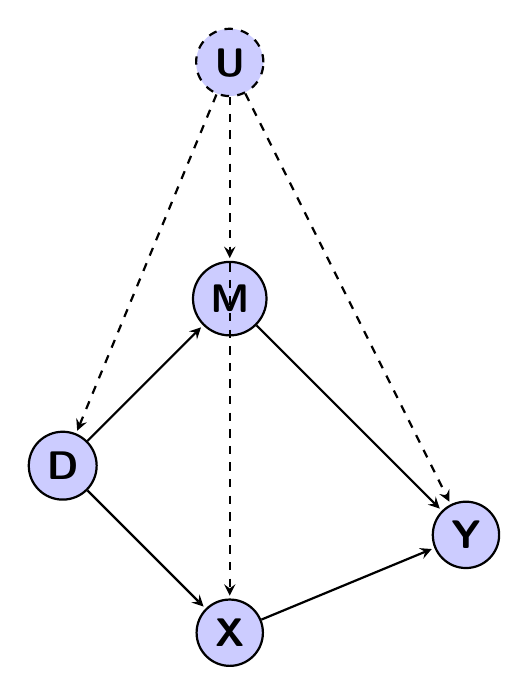
\begin{tikzpicture}[
  ->,>=stealth, % defines the style of the edge/arrow
  shorten >=1pt, % shortens the arrow at the target node
  auto,
  node distance=3cm, % defines the space between the nodes
  thick,
  main node/.style={circle,fill=blue!20,draw,font=\sffamily\Large\bfseries}, % style of the main nodes
  dashed node/.style={circle,fill=blue!20,draw,dashed,font=\sffamily\Large\bfseries} % style of the dashed node
  ]

  \node[main node] (D) {D}; 
  \node[main node] (M) [above right of=D] {M}; 
  \node[main node] (X) [below right of=D] {X};
  \node[main node] (Y) [right of=M, below of=M] {Y};
  \node[dashed node] (U) [above of=M] {U};
  
  \path[every node/.style={font=\sffamily\small}]
    (D) edge node {} (M)
    (D) edge node {} (X)
    (M) edge node {} (Y)
    (X) edge node {} (Y)
    (U) edge[dashed] node {} (D)
    (U) edge[dashed] node {} (M)
    (U) edge[dashed] node {} (X)
    (U) edge[dashed] node {} (Y);
\end{tikzpicture}

\end{frame}

\begin{frame}{Mechanism}

\begin{itemize}
\item $D$ is the treatment variable, and the ATT is over all possible channels, but what if you want to think $M$ is the mechanism
\item When you can't rule out competing theories with falsifications, you have to try and build the case that the effect is coming through a channel
\item Rule out $X$ and provide evidence for $M$
\item Goal here is to try and present evidence (not proof) that it's probably the story you're saying

\end{itemize}

\end{frame}



\begin{frame}{Ruling out alternative mechanism}

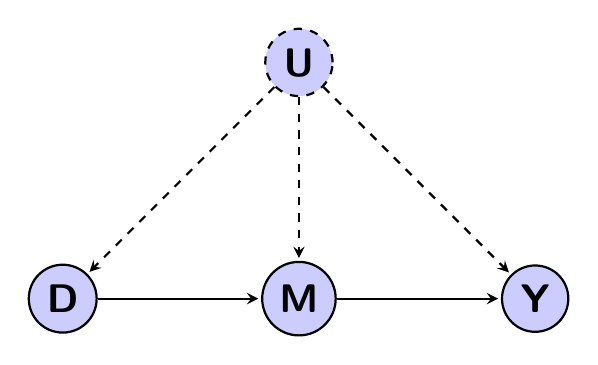
\begin{tikzpicture}[
  ->,>=stealth, % defines the style of the edge/arrow
  shorten >=1pt, % shortens the arrow at the target node
  auto,
  node distance=3cm, % defines the space between the nodes
  thick,
  main node/.style={circle,fill=blue!20,draw,font=\sffamily\Large\bfseries}, % style of the main nodes
  dashed node/.style={circle,fill=blue!20,draw,dashed,font=\sffamily\Large\bfseries} % style of the dashed node
  ]

  \node[main node] (D) {D}; 
  \node[main node] (M) [right of=D] {M}; 
  \node[main node] (Y) [right of=M] {Y};
  \node[dashed node] (U) [above of=M] {U};
  
  \path[every node/.style={font=\sffamily\small}]
    (D) edge node {} (M)
    (M) edge node {} (Y)
    (U) edge[dashed] node {} (D)
    (U) edge[dashed] node {} (M)
    (U) edge[dashed] node {} (Y);
\end{tikzpicture}


\end{frame}





\begin{frame}{Mechanism}

\begin{itemize}

\item Story is interpersonal comparisons which they try to show 
\item We can discuss how plausible we found it, but ask yourself at the end -- did the event study help you believe it?  Why/why not?

\end{itemize}

\end{frame}

\begin{frame}{Data on Facebook}

\begin{itemize}

\item Ingenious use of the Wayback Time Machine
\item Looked at over 700 schools using Facebook screen shots
\item When Facebook first mentions a school on its front page, that school is marked as having gotten Facebook

\end{itemize}

\end{frame}


\begin{frame}{New schools being adopted}
\begin{center}
\includegraphics[scale=0.35]{./lecture_includes/timemachine_1}
\end{center}
\end{frame}

\begin{frame}{New schools being adopted}
\begin{center}
\includegraphics[scale=0.35]{./lecture_includes/timemachine_2}
\end{center}
\end{frame}


\begin{frame}{Data on college students}

\begin{itemize}
\item NCHA Data is survey administered to college students on a semi-annual basis by American College Health Assoc
\item Inquires about demographics, physical health, mental health, alcohol and drug use, sexual behaviors, and perception of these behaviors by peers
\item ACHA merged a treatment indicator to each respondent based on Facebook dataset provided to them so that privacy could be maintained

\end{itemize}

\end{frame}

\begin{frame}{Mental health}

\begin{itemize}

\item Self-reported symptoms are standard medical practice in mental health -- DSM-5 relies on self-reports such as difficulty sleeping, fatigue, feelings of guilt, suicidal ideation
\item No data on Facebook or social media usage so this is ITT version of the ATT
\item Respondent answers to the questions are aggregated into indices such as \emph{poor mental health} where larger numbers are worse

\end{itemize}

\end{frame}

\begin{frame}{Main TWFE Model}

\begin{equation}
Y_{icgt} = \alpha_g + \delta_t + \beta \times Facebook_{gt} + X_i \times \gamma + X_c \times \psi + \varepsilon_{icgt}
\end{equation}

\bigskip

$Y_{icgt}$ is an outcome for person $i$ in wave $t$ attending college $c$ in expansion group $g$; $\alpha_g$ is expansion-group or college fixed effects; $\delta_t$ are survey-wave fixed effects; $Facebook_{gt}$ indicates the respondents' campus has Facebook by time $t$ at expansion group $g$; $X_i$ and $X_c$ are individual and college-level controls; and standard errors are clustered at college level.

\bigskip

$\widehat{\beta}$ identifies the ATT under parallel trends in the robust models


\end{frame}

\begin{frame}{Robustness}

\begin{itemize}

\item Main static results will all be in TWFE, but appendix shows other methods like CS and SA 
\item Event studies will show all models including some we haven't reviewed
\item Growing popularity to show ``all the robust DiD'' models so that readers can see you aren't cherry picking

\end{itemize}

\end{frame}



\begin{frame}
\begin{center}
\includegraphics[scale=0.35]{./lecture_includes/facebook_1}
\end{center}
\end{frame}

\begin{frame}
\begin{center}
\includegraphics[scale=0.35]{./lecture_includes/facebook_2}
\end{center}
\end{frame}

\begin{frame}
\begin{center}
\includegraphics[scale=0.35]{./lecture_includes/facebook_3}
\end{center}
\end{frame}

\begin{frame}
\begin{center}
\includegraphics[scale=0.35]{./lecture_includes/facebook_4}
\end{center}
\end{frame}

\begin{frame}
\begin{center}
\includegraphics[scale=0.35]{./lecture_includes/facebook_5}
\end{center}
\end{frame}

\begin{frame}
\begin{center}
\includegraphics[scale=0.35]{./lecture_includes/facebook_6}
\end{center}
\end{frame}

\begin{frame}
\begin{center}
\includegraphics[scale=0.35]{./lecture_includes/facebook_7}
\end{center}
\end{frame}

\begin{frame}{Conclusion}

\begin{itemize}
\item Good question, good data, and you can publish well with DiD
\item First evidence that social media caused mental health to worsen
\item Hardly definitive, but the staggered design is a solution to our inability to run the RCT
\item Remember -- many questions can be randomized in theory but not practice (e.g., smoking)
\item Clearly more work needs to be done, but this is a start
\end{itemize}

\end{frame}






\end{document}



\subsection{dCH}

\begin{frame}{de Chaisemartin and D'Haultfoeulle 2020}

de Chaisemartin and D'Haultfouelle 2020 (dCdH) is different from the other papers in several ways
	\begin{itemize}
	\item Like SA, it's a diagnosis and a cure
	\item TWFE decomposition shows coefficient a weighted average of underlying treatment effects, but weights can be negative negating causal interpretation
	\item Propose a solution for both static and dynamic specification which does not use already treated as controls
	\item Treatment can turn on and off
	\end{itemize}

\end{frame}


\begin{frame}{Comment on Bacon}

\begin{itemize}
\item Recall the Bacon decomposition -- TWFE coefficients are decomposed into weighted average of all underlying 2x2s. Weights were non-negative and summed to one.
\item But this decomposition was more a numerical decomposition -- what exactly adds up to equal the TWFE coefficient using the data we observe?
\item Bacon's decomposition is not ``theoretical'' -- not in the way that other decompositions are. He is just explaining what OLS ``does'' when it calculates $\widehat{\delta}$
\item Just explains what comparisons OLS is using to calculate the TWFE coefficient -- just peels back the curtain.
\end{itemize}

\end{frame}

\begin{frame}{Negative weights}

\begin{itemize}
\item dCdH impose causal assumptions and try a different decomposition strategy
\item Uses as its building block the unit-specific treatment effects
\item Their decomposition will reveal negative weights on the underlying treatment effects (similar to negative weight on dynamics with Bacon)
\item Remember though: the Bacon decomposition weights were \emph{always} positive, because they were numerical weights (not theoretical weights) on the underlying 2x2s (not the treatment effects)
\end{itemize}

\end{frame}

\begin{frame}{Turning on and off}

\begin{itemize}
\item CS and SA both require interventions to turn on and stay on
\item dCdH allows for ``switching'' on and off 
\item Before we move quickly into that, please note that the researcher bears the burden of knowing whether in fact you want to impose symmetry on turning on and off
\item Roe v Wade ``turned on'' legalized abortion and 2022 it was ``turned off'' -- do we want to treat these as simply a single policy flipping of the switch or two separate policies?
\end{itemize}

\end{frame}

\begin{frame}{dCdH notation}

\begin{itemize}
\item Individual treatment effects (iow, not the group-time ATT): $$\Delta^g_{i,t} = Y^1_{i,t} - Y^\infty_{i,t}$$ but where the treatment is in time period $g$. Notice --it's not the ATT (it's $i$ individual treatment effect)
\item with defined error term as $\varepsilon_{i,t}$: $$D_{i,t} = \alpha_i + \alpha_t + \varepsilon_{i,t}$$
\item Weights: $$w_{i,t} = \frac{\varepsilon_{i,t}}{\frac{1}{N^T} \sum_{i,t:D_{i,t}=1} \varepsilon_{i,t}}$$
\end{itemize}

\end{frame}

\begin{frame}{Parallel trend assumption}

\begin{block}{Strong unconditional PT}
Assume that for every time period $t$ and every group $g,g'$, $$E[Y^\infty_t - Y^\infty_{t-1}|G=g] = E[Y^\infty_t - Y^\infty_{t-1}|G=g'] $$
\end{block}Assume parallel trends for every unit in every cohort in every time period.

\bigskip

What then does TWFE estimate with differential timing?

\end{frame}

\begin{frame}{dCdH Theorem}

\begin{block}{Theorem -- dCdH decomposition}
Assuming SUTVA, no anticipation and the strong PT, then let $\delta$ be the TWFE estimand associated with $$Y_{i,t} = \alpha_i + \alpha_t + \delta D_{i,t} + \varepsilon_{i,t}$$Then it follows that $$\delta = E \bigg [ \sum_{i,t:D_{i,t}=1} \frac{1}{N^T} w_{i,t} \cdot \Delta_{i,t}^g \bigg ] $$ where $\sum_{i,t:D_{i,t}=1} \frac{w_{i,t}}{N^T} = 1$ but $w_{i,t}$ can be negative
\end{block}

\end{frame}

\begin{frame}{Origins}

\begin{itemize}
\item So once you run that specification, $\widehat{\delta}$ is going to recover a ``non-convex average'' over all unit level treatment effects (weights can be negative, more on this). 
\item Not sure who came first, because there were working papers before publications, but my understanding is dCdH was the first to prove this
\item Very important theorem -- established the ``no sign flip property'' for OLS with differential timing in the canonical static specification
\end{itemize}

\end{frame}


\begin{frame}{Negative weights}

\begin{itemize}
\item Very common now to hear about negative weights, and furthermore, that negative weights wipe out any causal interpretation, but why?
\item Thought experiment: imagine every unit gained from the treatment, but their treatment effect when estimated was multiplied by a negative number
\item It's possible it could flip the sign, but it would definitely at least pull the estimate away from the true effect
\item This is dangerous -- and it's caused by the forbidden contrasts (comparing treated to already treated) which is what the canonical TWFE static specification is doing (for many of us unknowingly)
\end{itemize}

\end{frame}



\begin{frame}{Negative weights}

\begin{itemize}
\item Doesn't always pose a problem, but no proofs for this intuition known yet
\item A large number of never-treated seems to make this less an issue
\item Shrinking the spacing between treatment dates also can drive it down
\item But does that mean that TWFE works, and what does it mean to work?
\item TWFE still even when all the weights are positive the weighted average may not aggregate to what we think it does
\end{itemize}

\end{frame}

\begin{frame}{Weighting}

\begin{itemize}
\item The weights in OLS all come out of the model itself, \emph{not the economic question}
\item The economic question is ``what parameter do you want? What does it look like? Who is in it?''
\item And when you define the parameter up front, you've more or less defined the economic question you're asking
\item But OLS sort of ignores your question and just gives you what it wants
\end{itemize}

\end{frame}

\begin{frame}{Weighting}

\begin{itemize}
\item What makes something a good vs a bad weight?
\item Not being negative is the absolute minimal requirement
\item But it's also not a good sign if you can't really explain the weights
\end{itemize}

\end{frame}

\begin{frame}{dCdH Solution}

\begin{itemize}
\item dCdH propose an alternative that doesn't have the problems of TWFE -- both avoiding negative weights and improving interpretability
\item Recall, their model can handle reversible treatments

\end{itemize}

\end{frame}

